%!TEX program = xelatex
% 完整编译: xelatex -> biber/bibtex -> xelatex -> xelatex
\documentclass[lang=cn,a4paper,newtx,bibend=bibtex]{elegantpaper}

\title{Theoretical Questions of Chapter 1}
\author{张志心 \ 计科2106}

\date{\zhdate{2023/09/26}}

% \qedhere to make the square straight after

\usepackage{array}
\usepackage{tcolorbox}
\usepackage{tikz}
\usepackage{pgfplots}

\newtcolorbox{prob}[1][]{
  colframe=gray,
  colback=white,
  boxrule=1.5pt, % 控制外边框线的宽度
  sharp corners, % 使用直角边框
  fonttitle=\bfseries,
  title=#1
}

\newcommand{\ccr}[1]{\makecell{{\color{#1}\rule{1cm}{1cm}}}}

\addbibresource[location=local]{reference.bib}

\begin{document}

\maketitle



\begin{prob}[1.8.1-\textrm{I}.]
Consider the bisection method starting with the ini-
 tial interval $[1.5, 3.5]$. In the following questions “the
 interval” refers to the bisection interval whose width
 changes across different loops.
 \begin{itemize}
    \item What is the width of the interval at the $n$-th step?
    \item What is the supremum of the distance between
    the root $r$ and the midpoint of the interval?
 \end{itemize}
\end{prob}

\begin{solution}
    二分法每次让搜索区间减半,因此 $b_n-a_n = 2^{-n}(b_0 - a_0) = 2^{-(n-1)}$ ;
    由于 $x^* \in [a_n, b_n]$,所以 $\vert x^* - \dfrac{a_n + b_n}{2}\vert \le \dfrac12 \vert b_n - a_n\vert = 2^{-n}$。
\end{solution}

\begin{prob}[1.8.1-\textrm{II}.]
    In using the bisection algorithm with its initial interval
    as $[a_0, b_0]$ with $a_0 > 0$, we want to determine the root
    with its relative error no greater than $\epsilon$. Prove that this
    goal of accuracy is guaranteed by the following choice
    of the number of steps,

    \[
        n\ge \dfrac{\log(b_0 - a_0)-\log \epsilon - \log a_0}{\log 2} - 1.
    \]

\end{prob}
    
\begin{proof}
设根为 $r>0,r\in[a_0, b_0]$,由于 $\epsilon \ge \dfrac{\vert\frac{a_n+b_n}{2}-r\vert}{r}$
。而 $\vert\frac{a_n+b_n}{2}-r\vert \le \frac{b_0-a_0}{2^{n+1}}$,
若使
\[
    \dfrac{\vert\frac{a_n+b_n}{2}-r\vert}{r}\le \frac{b_0-a_0}{2^{n+1}a_0} \le \epsilon,
\]
则结论可满足,所以
\[
    2^{n+1}\ge \dfrac{b_0-a_0}{a_0\epsilon} \Rightarrow
    n\ge \log_2 {\dfrac{b_0-a_0}{a_0\epsilon}} - 1 = \dfrac{\log(b_0-a_0)-\log \epsilon-\log a_0}{\log 2}-1.
\]
\end{proof}


\begin{prob}[1.8.1-\textrm{III}.]
        Perform four iterations of Newton’s method for the
        polynomial equation $p(x) = 4x^3 - 2x^2 + 3 = 0$ with
 the starting point $x_0 = -1$. Use a hand calculator and
organize results of the iterations in a table.
\end{prob}
        
\begin{solution}
    $p'(x) = 12x^2-4x, p(x) = 4x^3 - 2x^2 + 3$,根据牛顿法,$x_{n+1}=x_n-\dfrac{p(x_n)}{p'(x_n)}$。

    \begin{center}
        \begin{tabular}{|c|c|c|c|}
        \hline
        Iteration & \(x_n\) & \(p(x_n)\) & \(p'(x_n)\) \\
        \hline
        0 & -1 & -3 & 16 \\
        1 & -0.8125 & -0.465820 & 11.1719 \\
        2 & -0.770804 & -0.020138 & 10.2129 \\
        3 & -0.768832 & -0.000044 & 10.1686 \\
        4 & -0.768828 & 2e-10 & 10.1685 \\
        \hline
        \end{tabular}
    \end{center}          
\end{solution}
    
\begin{prob}[1.8.1-\textrm{IV}.]
    Consider a variation of Newton’s method in which only
    the derivative at $x0$ is used,
    \[
    x_{n+1}=x_n-\frac{f(x_n)}{f'(x_0)}.
    \] 
    Find $C$ and $s$ such that $e_{n+1}=Ce_n^s$, 
    where en is the error of Newton’s method at step $n$, $s$ is
    a constant, and $C$ may depend on $x_n$, the true solution
    $\alpha$, and the derivative of the function $f$.
\end{prob}
        
\begin{solution}
设根为 $r$,由变种牛顿迭代的公式可的得
\[
e_{n+1}=\vert x_{n+1}-r\vert = \vert x_{n}-r-\dfrac{f(x_n)}{f'(x_0)} \vert = \vert x_n-r\vert \bigg\vert 1-\dfrac{f(x_n)}{f'(x_0)(x_n-r)}\bigg\vert    
\]
所以 $s=1,C=\bigg\vert 1-\dfrac{f(x_n)-f(r)}{f'(x_0)(x_n-r)}\bigg\vert$.
\end{solution}

\begin{prob}[1.8.1-\textrm{V}.]
    Within $(-\frac{\pi}2,\frac{\pi}2)$, will the iteration
    $x_{n+1}=\tan^{-1}x_n$ converge?
\end{prob}
        
\begin{solution}
收敛,理由如下:由于 $(\tan^{-1}x - x)'=\frac{1}{1+x^2}-1 < 0$,所以 $\tan^{-1}x -x$ 单调递减,
又因为 $\tan^{-1}0 - 0 = 0$,所以当 $x<0$ 时,$\tan^{-1}x > x$,当 $x>0$ 时候,$\tan^{-1}x < x$。
因此,当 $x_0 = 0$ 时,显然 $x_n\equiv 0$,因此迭代收敛;当 $x\in(-\frac{\pi}{2},0)$ 时,
$x_n < x_{n+1} < 0$,根据单调收敛定理,迭代收敛;同理,当 $x\in(0,\frac{\pi}{2})$ 
,$x_n > x_{n+1} > 0$,根据单调收敛定理,迭代收敛。
\end{solution}

\begin{prob}[1.8.1-\textrm{VI}.]
    Let $p\ge 1$. What is the value of the following continued
    fraction?
    \[
        x=\frac{1}{p+\frac{1}{p+\frac{1}{p+\cdots}}}.
        \]
    Prove that the sequence of values converges. (Hint:
    this can be interpreted as $x = \lim_{n\to +\infty} x_n$, where
    $x_1 = \dfrac1p,x_2=\dfrac{1}{p+\frac1p}, \cdots$,and so forth.
    Formulate $x$ as a fixed point of some function.)
\end{prob}
        
\begin{solution}
问题等价于求解 $x = \lim_{x\to +\infty} x_n$,其中,$x_1 = 0, x_{n+1} = \dfrac{1}{p + x_n} (n \ge 1)$。
又因为 $(\dfrac{1}{p+x})'=\dfrac{-1}{(p+x)^2} \le \dfrac{1}{p^2} < 1 (x \ge 0)$,
根据压缩映射的性质,$\{x_n\}$ 收敛于 $ x=\dfrac{1}{p+x}$,所以 $x=\dfrac{-p+\sqrt{p^2+4}}{2}$(舍去负数值)。
所以该连分数的值为 $\dfrac{-p+\sqrt{p^2+4}}{2}$。
\end{solution}

\begin{prob}[1.8.1-\textrm{VII}.]
    What happens in problem \textrm{II} if $a_0 < 0 < b_0$? Derive
    an inequality of the number of steps similar to that in
    \textrm{II}. In this case, is the relative error still an appropriate
    measure?
\end{prob}
        
\begin{solution}
    由\textrm{II}可知,$\dfrac{\vert\frac{a_n+b_n}{2}-r\vert}{\vert r\vert }\le \frac{b_0-a_0}{2^{n+1}\vert r\vert }$,
    因此有 $n\ge \log_2 {\dfrac{b_0-a_0}{a_0\epsilon}} - 1 = \dfrac{\log(b_0-a_0)-\log \epsilon-\log {\vert r\vert}}{\log 2}-1$,
    然而由于 $\vert r\vert$ 可以无限小,所以相对误差可以无限大,
    特别的,当 $r = 0$ 时,相对误差无意义,因此相对误差不再是可估计的。
\end{solution}

\begin{prob}[1.8.1-\textrm{VIII}.]
    (*) Consider solving $f(x) = 0 (f \in \mathcal{C}^{k+1})$ by Newton’s
method with the starting point $x_0$ close to a root of
multiplicity $k$. Note that $\alpha$ is a zero of multiplicity $k$
of the function $f$ iff
\[f^{(k)}(\alpha) \neq 0; \forall i < k, f^{(i)}(\alpha) = 0.\]
\begin{itemize}
\item How can a multiple zero be detected by examining
the behavior of the points $(x_n, f(x_n))$?
\item Prove that if $r$ is a zero of multiplicity $k$ of the
function $f$, then quadratic convergence in Newton’s iteration will be restored by making this
modification:
\[
    x_{n+1}=x_n-k\dfrac{f(x_n)}{f'(x_n)}.
    \]
\end{itemize}
\end{prob}
        
\begin{solution}
函数在重根处的一阶导为 $0$,而在单根处的一阶导不为 $0$。
可以通过观察函数图像在零点处的斜率来判断是否为重根。例如 $f(x) = (x+3)(x+1)^3(x-2)^2$ ,
根据下图可以很容易判断出,$x=-1,2$ 为重根,而 $x=-3$ 为单根。
\begin{center}
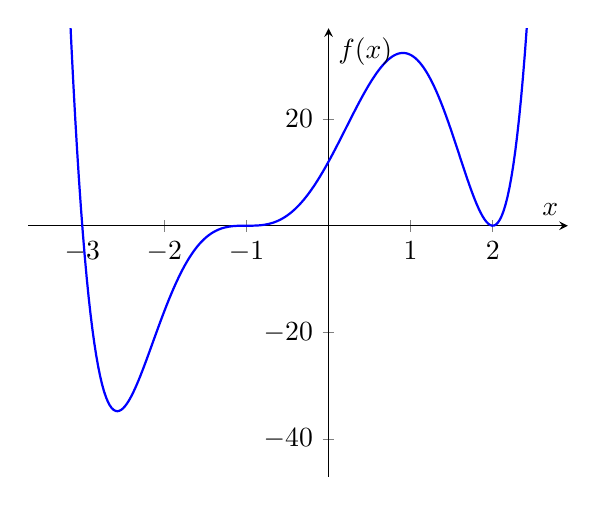
\begin{tikzpicture}
    \begin{axis}[
        xlabel=$x$,
        ylabel=$f(x)$,
        ymin=-40, ymax=30,
        domain=-4:3,
        samples=300,
        axis lines=middle,
        enlargelimits=true,
    ]
    \addplot[blue, thick] {(x+3)*(x+1)^3*(x-2)^2};
    \end{axis}
\end{tikzpicture}
\end{center}
\end{solution}


对于求解 $k$ 重根的牛顿迭代法,\\

设 $f(x)=g(x)(x-x^*)^k, g(x^*) \neq 0, f\in \mathcal{C}^{k+1} \Rightarrow g\in \mathcal{C}^1$,那么
\[
    x_{n+1} = x_n - \dfrac{kg(x_n)(x_n-x^*)^k}{kg(x_n)(x_n-x^*)^{k-1}+g'(x_n)(x_n-x^*)^k}
    = x_n - \dfrac{kg(x_n)(x_n-x^*)}{kg(x_n)+g'(x_n)(x_n-x^*)}.
\]
所以,
\begin{equation*}
    \begin{aligned}
        x_{n+1} - x^* &= x_n - x^* -  \dfrac{kg(x_n)(x_n-x^*)}{kg(x_n)+g'(x_n)(x_n-x^*)} \\
                      &= (x_n - x^*) \bigg(1 -  
                        \dfrac{kg(x_n)}{kg(x_n)+g'(x_n)(x_n-x^*)}
                        \bigg) \\
                    &= (x_n - x^*) \bigg(
                    \dfrac{g'(x_n)(x_n-x^*)}{kg(x_n)+g'(x_n)(x_n-x^*)}
                    \bigg) \\
                    &= (x_n - x^*)^2 \bigg(
                        \dfrac{g'(x_n)}{kg(x_n)+g'(x_n)(x_n-x^*)}
                        \bigg). \\
    \end{aligned}
\end{equation*}

所以 $\vert x_{n+1} - x^*\vert = \vert x_n - x^*\vert^2 \bigg\vert 
\dfrac{1}{k\dfrac{g(x_n)}{g'(x_n)} + (x_n - x^*)}
\bigg\vert$,

当 $\vert x_0-x^* \vert < \bigg\vert\dfrac{k\min_{x\in \mathcal{D}_f}{g(x_n)}}{\max_{x\in \mathcal{D}_f}{g'(x_n)}}\bigg\vert - \epsilon$ 时,
该迭代方法二阶收敛。



% \nocite{*}
% \printbibliography[heading=bibintoc, title=\ebibname]

% \appendix
% % \appendixpage
% \addappheadtotoc

\end{document}
